\chapter{Python 概述与安装}
\section{Python 的发展历史与应用}
Python 的诞生时间非常早,第一版 Python 发行于 1991 年,甚至比 Java 的历史都早。在大部分时间内,Python 一直作为一个小众的编程语言,并没有大规模流行起来。近些年来,随着大数据技术、人工智能技术的发展和普及,“简洁、具有良好扩展性”的 Python 非常契合大数据与人工智能技术对编程语言的要求,超越其他编程语言迅速崛起。Python 分别在2010年,2018年被全球知名的编程语言流行度排行榜网站 TIOBE 评为“年度最佳编程语言”,并长期位于各年或各月流行编程语言排行榜的前三名。中国的网络上甚至产生了一句流行语:“人生苦短,我用 Python”。

Python 的创始人为荷兰人吉多·范罗苏姆(Guido van Rossum),在 1989 年的圣诞节期间,吉多·范罗苏姆为了打发时间,决心开发一个新的脚本解释程序,作为 ABC语言的继承,于是 Python 诞生了。之所以选择 Python 作为名字,是由于吉多·范罗苏姆非常喜欢一部 BBC 电视剧--- Monty Python's Flying Circus(中文译名:蒙提·派森的飞行马戏团)。 Python 的英文意思为蟒蛇,这也是为什么一些 Python 相关的软件或书籍用蟒蛇作为图标的原因。

Python的设计哲学是“优雅”、“明确”、“简单”,Python 可以说是语法功能最简单的编程语言之一。Python具有良好的可扩展性,Python提供了丰富的接口和工具,以便程序员能够轻松地使用 C、C++、Cython来编写扩展模块,因此,有很多人把Python作为一种“胶水语言”使用。Python是完全面向对象的语言,函数、模块、数字、字符串都是对象,并且完全支持继承、重载、派生、多重继承等,Python 还支持重载运算符。并且随着计算机速度运算速度越来越快,Python 运算速度慢的缺点逐渐可以忽略,因此,许多网站开始使用 Python 开发,许多专业软件也开始支持 Python 调用。

Python 的应用范围包括 Web 开发网站与网络爬虫,GUI 开发桌面软件,科学计算等。使用Python编写的著名应用包括:

\vspace{5pt}
\begin{itemize}
  \item Youtube --- 视频分享网站

  \item Dropbox --- 文件分享软件

  \item Instagram --- 图片分享软件


  \item 豆瓣网 --- 国内著名的图书、唱片、电影评论网站

  \item 知乎网 --- 国内著名的问答网站

  \item 果壳网 --- 国内著名的泛科技主题网站
\end{itemize}
\vspace{5pt}

目前的主要 Python 版本为 Python3,本书的所有 Python 程序都是 Python3 版本。

\clearpage
\section{安装 Python}

使用 Python 时一般有两种方式:一是下载 Python 和编辑器 Pycharm,二是下载 Anaconda(自带 Python) 和编辑器 Spyder。从实践经验来看,Pycharm 功能 比 Spyder 更多,更加人性化,笔者优先推荐第一种方式。

\subsection{Python + Pycharm}
\subsubsection{下载python}


Python 的官方网址为:\href{https://www.python.org}{https://www.python.org}。打开网址后,从 Download 里面可以找到不同操作系统的 python 版本下载。下面我们以 Windows 系统为例讲述 Python 的安装。

\begin{figure}[!ht]
  \centering
  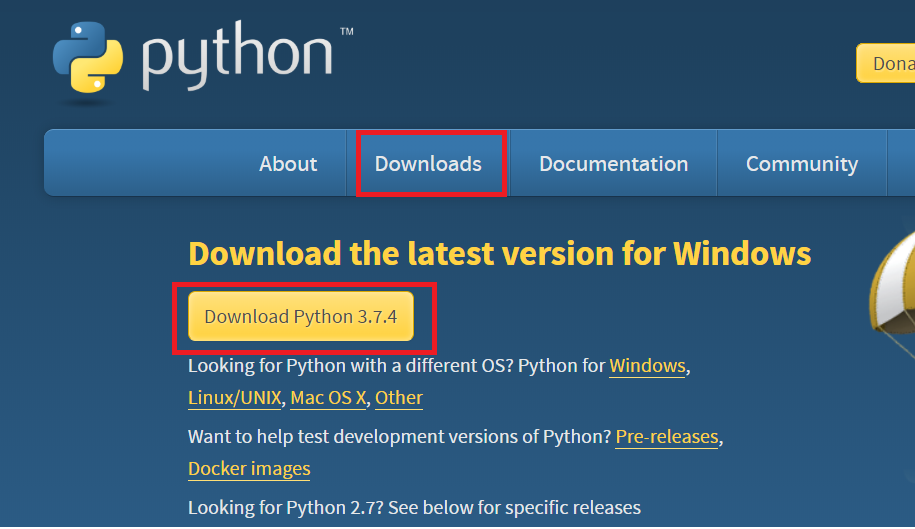
\includegraphics[scale=0.6]{figure/chapter1/pythonDownload.png}
\end{figure}

下载完成后,双击 exe 文件安装,切记要勾选 Add Python 3.7 to PATH, 然后点击 Install Now(默认安装目录,默认安装 pip 等)或 Customize installation(可以自己设置安装目录等)都可以。

\begin{figure}[ht]
  \centering
  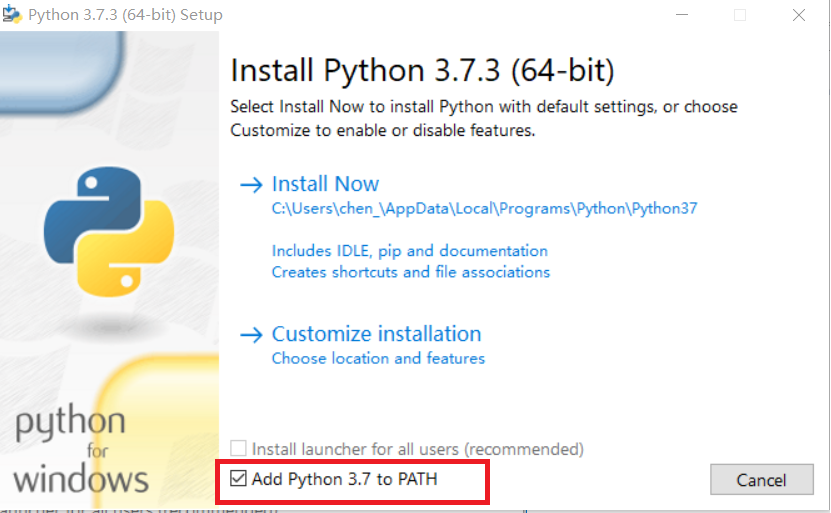
\includegraphics[scale=0.6]{figure/chapter1/pythonDownload2.png}
\end{figure}

为了测试 Python 是否安装成功,打开命令行窗口(win10 系统中敲 win 健,再输入 cmd,然后回车),输入 python,若能显示 Python 的版本信息,则代表 python 已正确安装。

\begin{figure}[!ht]
  \centering
  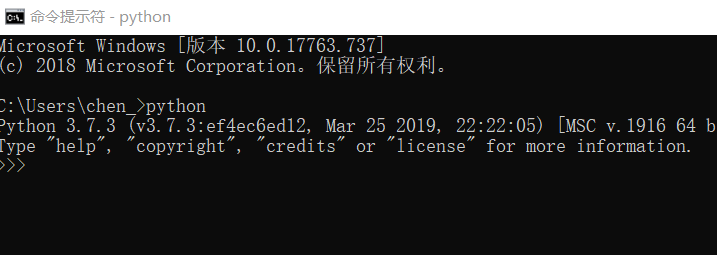
\includegraphics[scale=0.7]{figure/chapter1/pythonDownload3.png}
\end{figure}

\subsubsection{下载 Pycharm}


Pycharm 的官方网址:\href{http://www.jetbrains.com/pycharm}{http://www.jetbrains.com/pycharm},点击 DOWNLOAD 开始安装。

\begin{figure}[!ht]
  \centering
  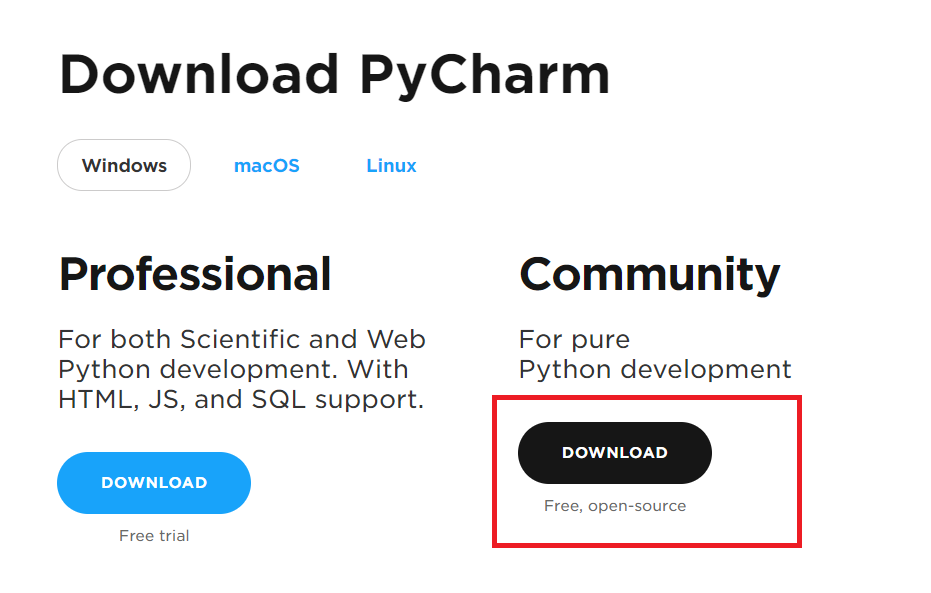
\includegraphics[scale=0.6]{figure/chapter1/pycharm.png}
\end{figure}

一般选择免费版本下载,下载完成后双击 exe 进行安装。

\begin{figure}[!ht]
  \centering
  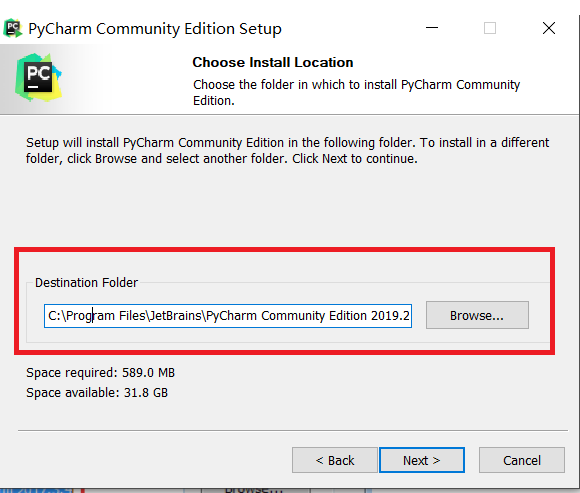
\includegraphics[scale=0.6]{figure/chapter1/pycharm2.png}
\end{figure}

可以通过图中的 Browse 更改安装目录,其他步骤按照默认设置即完成安装。

完成安装后,设置 Pycharm 中的 Python 解释器为我们安装的 Python 版本。打开 Pycharm, 依次点击 file--settings--project interpreter,将 interpreter 设置为Python 安装路径中的 python.exe(笔者电脑的位置为 \path{D:\python:\python.exe})。

\begin{figure}[!ht]
  \centering
  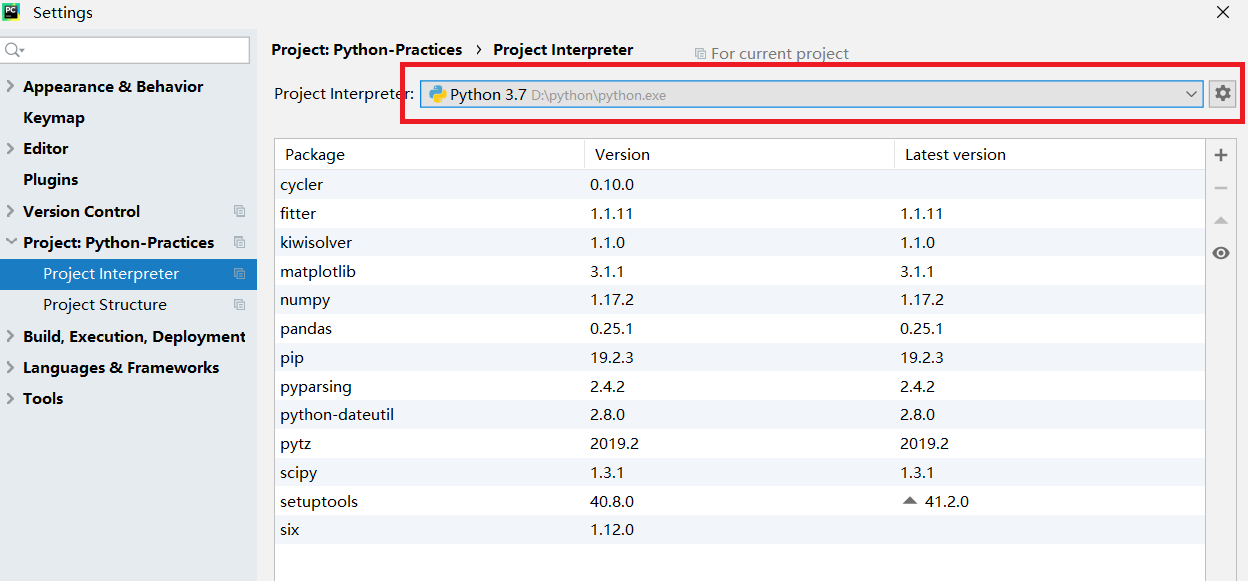
\includegraphics[scale=0.4]{figure/chapter1/pycharm3.png}
\end{figure}



\subsection{Anaconda + Spyder}

\section{统计学常用 Python 包的安装}
